\chapter{Predicting the unbiased MET Distribution at Higher Luminosity}
\section{Objective}
Our goal is to empirically reconstruct the unbiased CELL MET distribution using \texttt{HLT\_noalg\_L1ZB}, \texttt{HLT\_noalg\_L1XE30} and \texttt{HLT\_noalg\_L1XE50} data. By this data, I mean the events for which these triggers fired. The \texttt{HLT\_noalg\_L1XExx} triggers are triggers that fire randomly, but only select events that have L1 MET greater than xx. 
As a result, the data selected by these triggers are biased with respect to L1 (except for the \texttt{HLT\_noalg\_L1ZB}). 
However, we want to use this data to determine the CELL MET distribution as a function of $\mu$.
Because the ZeroBias events only allow us to go up to about $80$ GeV, we use the \texttt{HLTnoalg\_L1XExx} triggered events in order to extend to higher MET. This is important because knowing the distribution of MET as determined by the CELL algorithm as a function of $\mu$ helps us to better understand the background rate of events and allows us to test models for this rate. This allows us to get a better handle on predicting what kind of rates of events we'll need to account for when designing the triggers and how the increasing luminosity could affect the efficiency of the trigger system.
As a result of the bias with respect to L1, in order to get the unbiased distribution, we must correct the \texttt{HLTnoalg\_L1XExx} data using the efficiency curves determined from lower threshold triggers back to ZeroBias.
While performing this correction, it was important to propagate the errors due to the determination in the efficiency, and those due to statistical uncertainties.
Performing the reconstruction involved several steps:
\begin{enumerate}
        \item compute the efficiency of $L1>30$GeV for \texttt{HLT\_ZB\_L1ZB} data as a function of CELL MET
        \item correct the \texttt{HLT\_ZB\_L1XE30} data back to the \texttt{HLT\_ZB\_L1ZB} distribution by multiplying by the prescale and dividing by the efficiency. 
        \item compute the efficiency of $L1>50GeV$ for \texttt{HLT\_ZB\_L1XE30} data as a function of CELL MET
        \item correct the \texttt{HLT\_ZB\_L1XE50} data back to the \texttt{HLT\_ZB\_L1ZB} distribution by multiplying by the corresponding prescale, and dividing by both of the previously computed efficiencies. 
\end{enumerate}
For this project, we used the 2015, 2016 and 2017 combined \texttt{HLTnoalg\_L1ZB} , \texttt{HLTnoalg\_L1XE30} and \texttt{HLTnoalg\_L1XE50} data produced by Jonathan Burr on 11/17/2017 from the zerobias and JETM10 trees.
In addition, we removed the events from runs 330203, 331975 and 334487 because these events had large MET events without jets and the logbook says there were calorimeter noise problems in these runs. 

\section{Efficiency Fits}
It was necessary to come up with a model that could be used to fit to our efficiency data. To create this model, we assumed that the conditional distribution of the value of MET as determined by L1, given the value of MET as determined by CELL was a gaussian:
\begin{align}
		\mathbb{P}(X=x|Y) = \frac{1}{\sigma \sqrt{2\pi}} e^{-z^2/2\sigma^2}
\end{align}
Where we have defined:
\begin{align}
		z=y-(ax+b)
\end{align}
Then, in order to derive the expression for the model for the efficiency curves, we compute the probability that L1 determines as MET value higher than the value of the threshold. In order to do this, we integrate from the value of the threshold ($T$) to infinity:
\begin{align}
		\varepsilon(x)=\frac{1}{\sigma \sqrt{2\pi}}\int_{T}^{\infty}e^{-z^2/2\sigma^2}dz
\end{align}
One may manipulate this expression using properties of integration, probability density functions and gaussians in order to write an expression for the efficiency in terms of the error function:
\begin{align}
		\textrm{Erf}(z)=\frac{2}{\sqrt{\pi}}\int_0^{z}e^{-t^2}dt
\end{align}
Finally, the expression we get is:
\begin{align}
		\varepsilon(x)=\frac{1}{2}\left( 1+\textrm{Erf}\left( \frac{ax+b-T}{\sigma\sqrt{2}} \right) \right)
\end{align}
We performed this fit for the distribution of MET in $\mu$ bins of $0-10,\ldots,60-70$
\pagebreak
\begin{figure}[h]
		\centering
		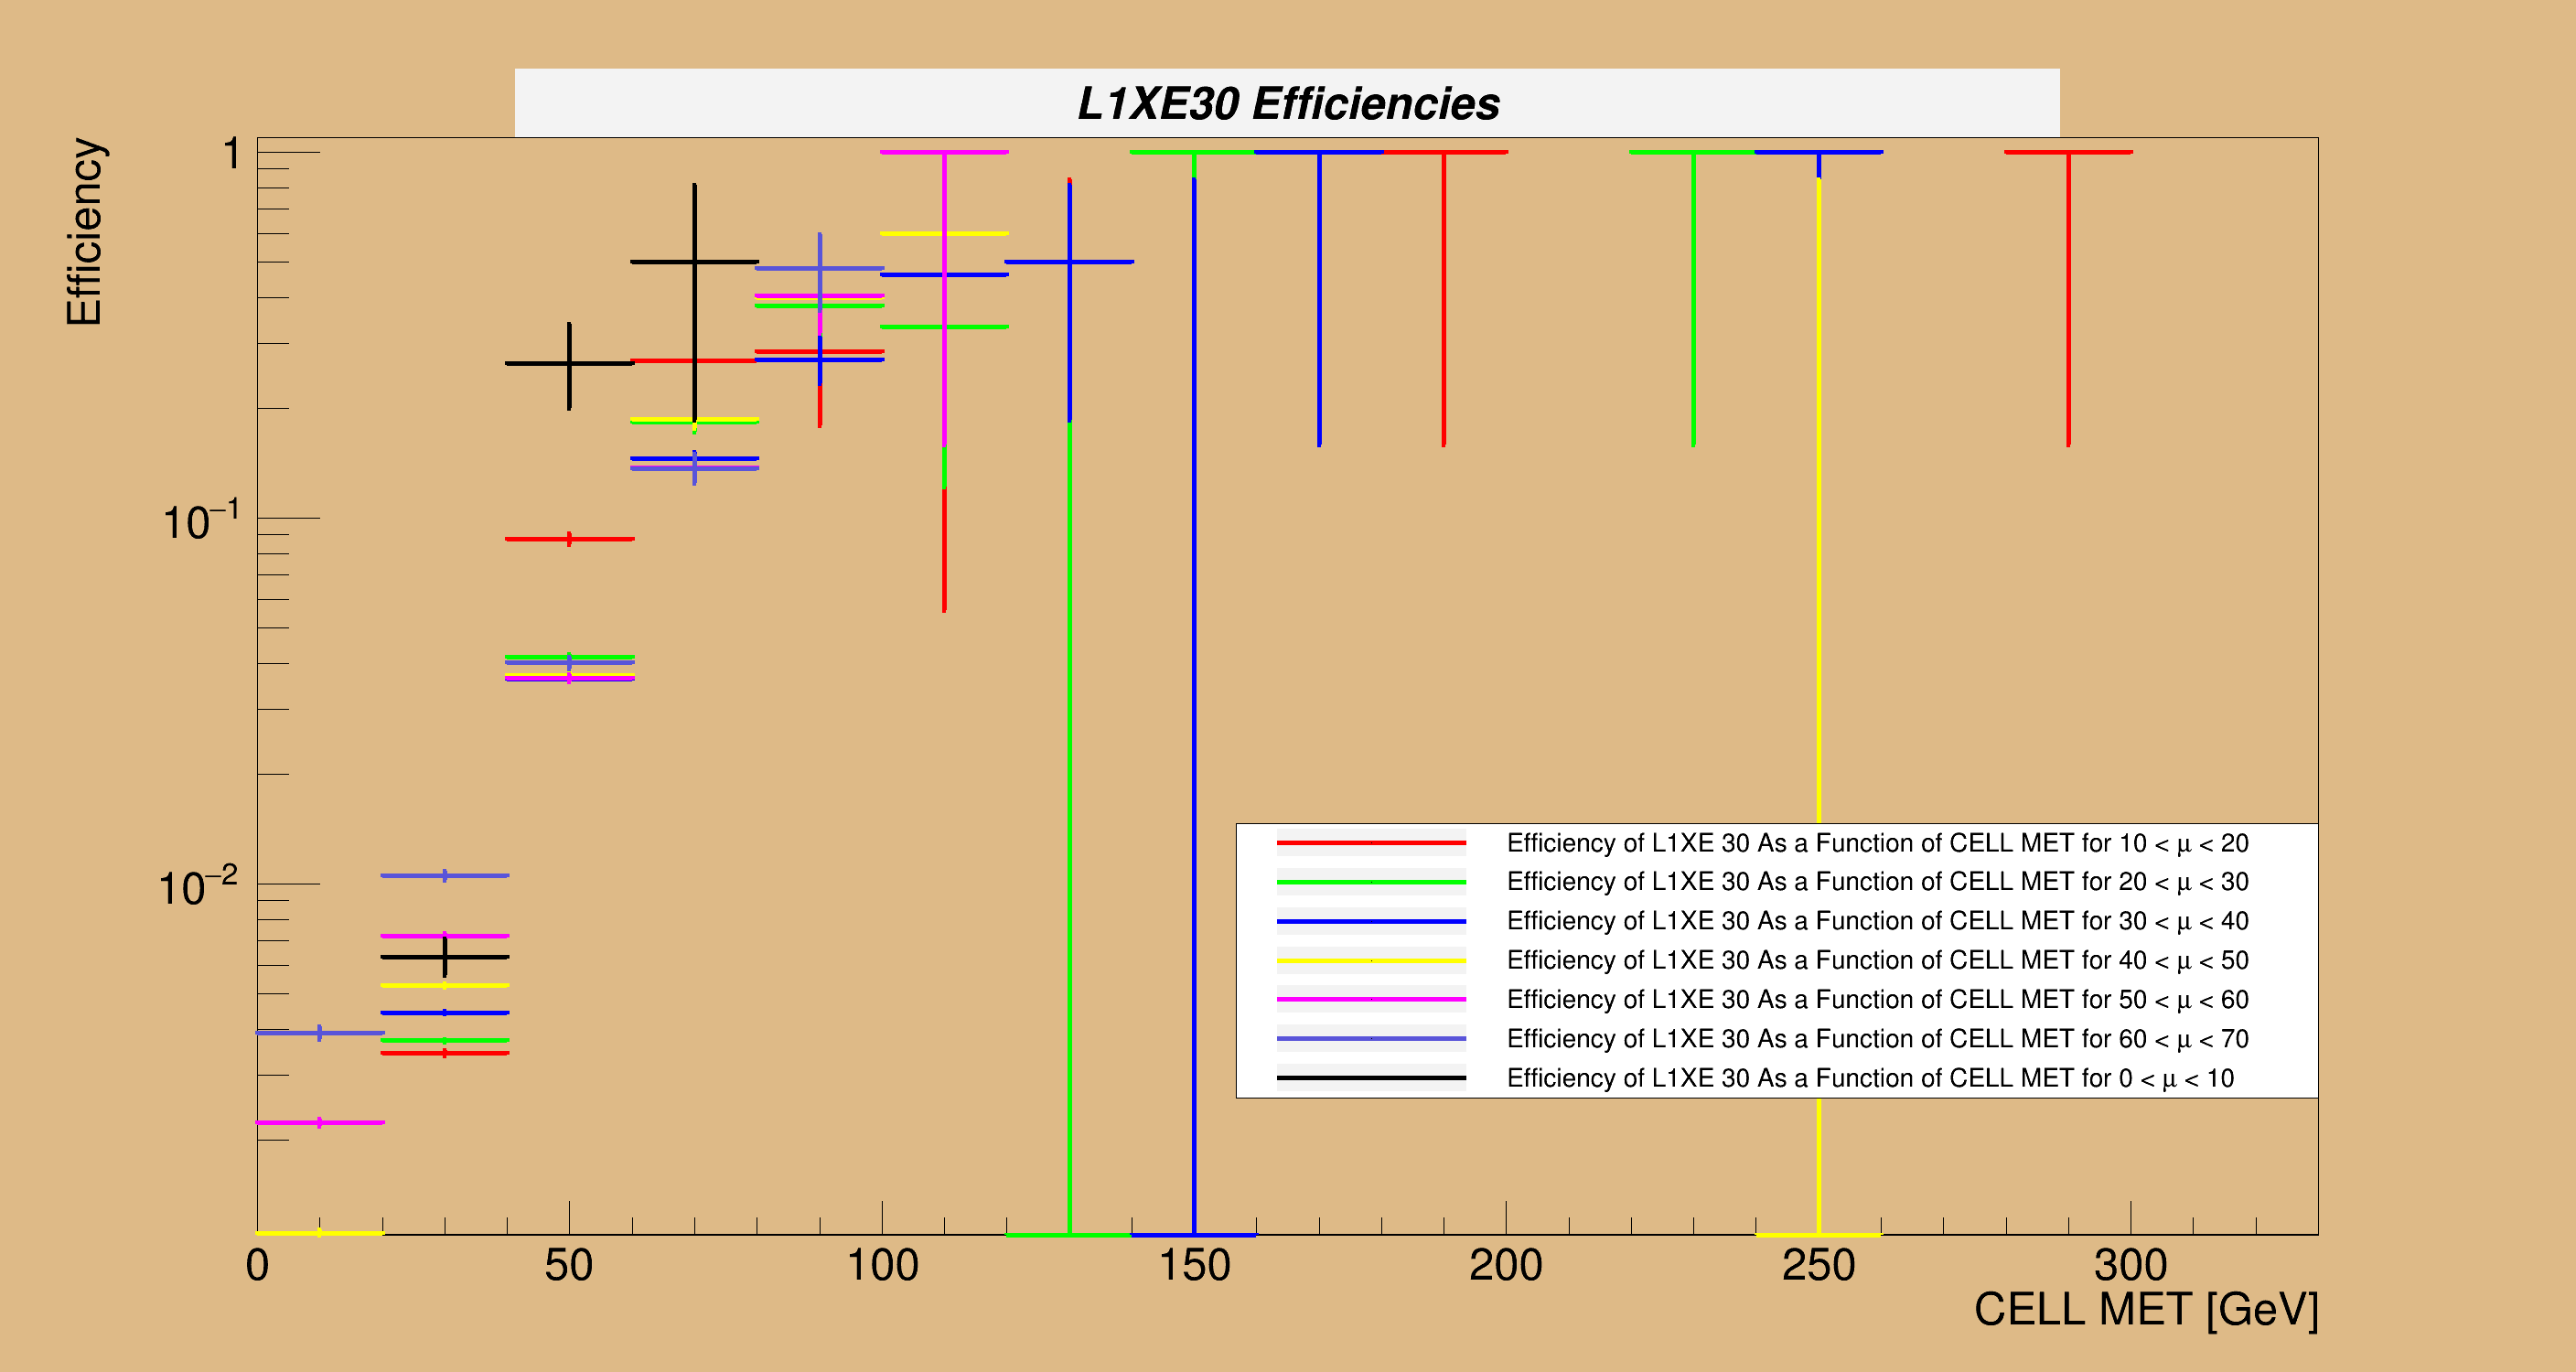
\includegraphics[scale=0.12]{L1XE30Efficiency_Curves}
		\caption{Efficiency Curves of L1$>30$ on the \texttt{HLT\_noalg\_L1ZB} data}
\end{figure}
\begin{figure}[h]
		\centering
		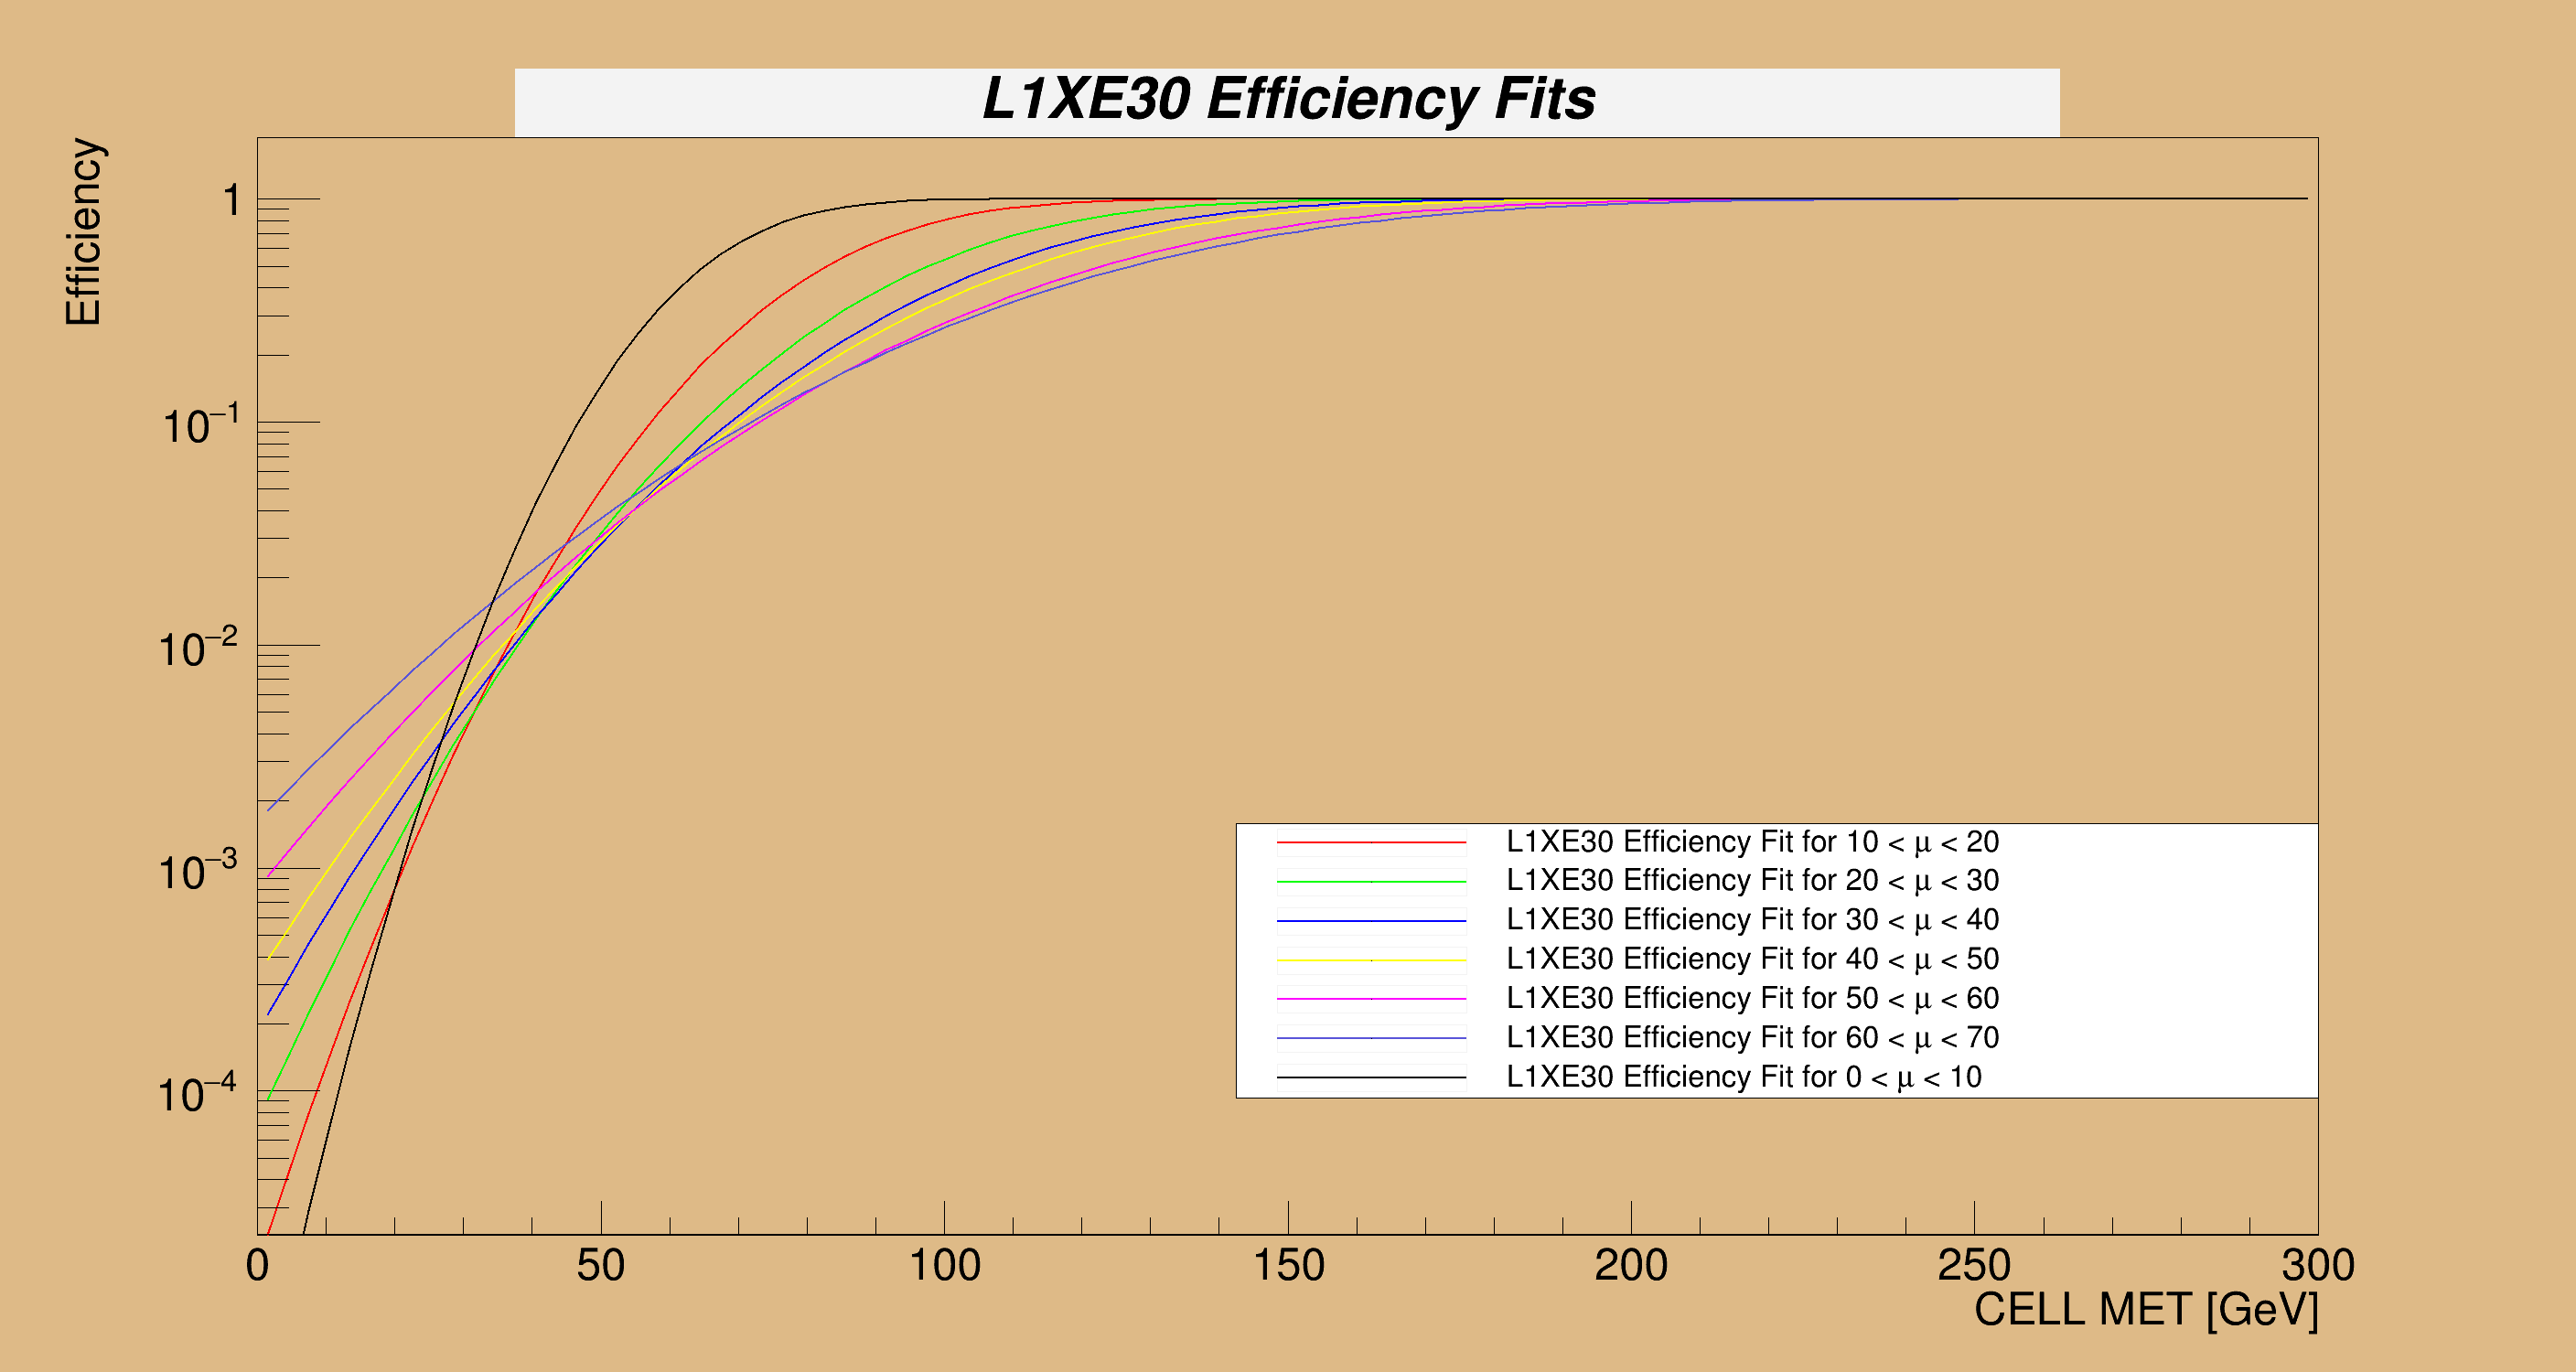
\includegraphics[scale=0.15]{L1XE30Efficiency_Fits}
		\caption{Efficiency Curves of L1$>30$ on the \texttt{HLT\_noalg\_L1ZB} data}
\end{figure}
\begin{figure}[h]
		\centering
		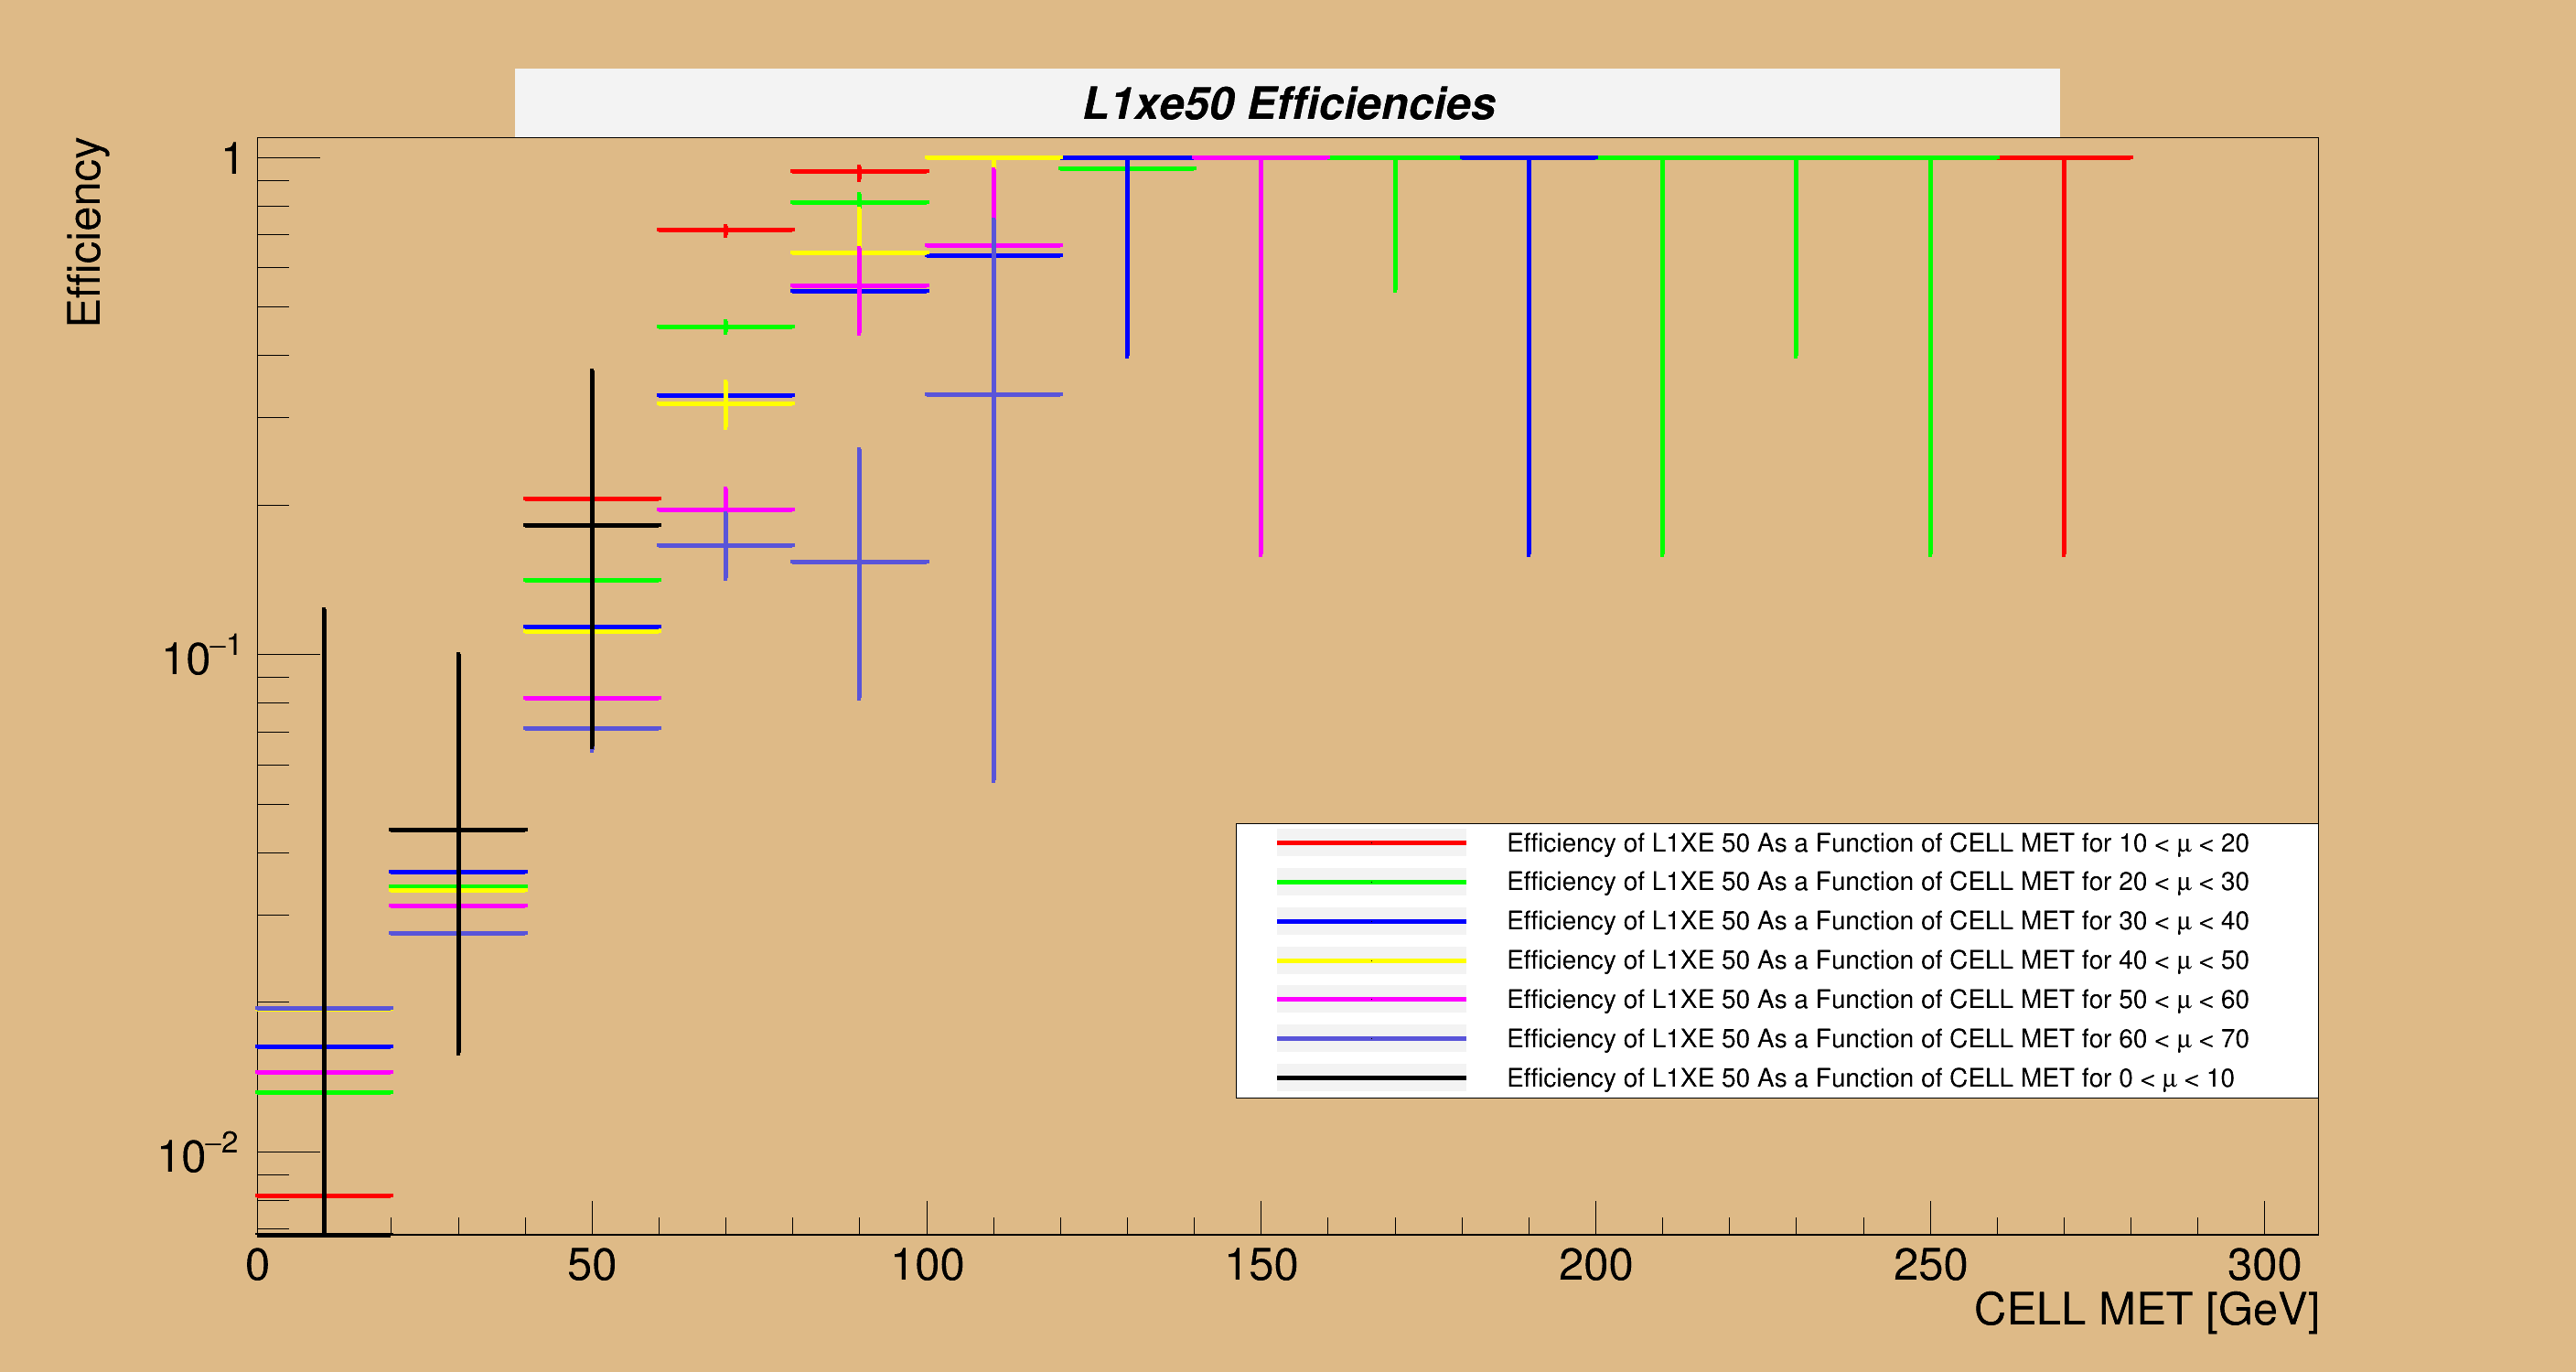
\includegraphics[scale=0.15]{L1XE50Efficiency_Curves}
		\caption{Efficiency Curves of L1$>50$ on the \texttt{HLT\_noalg\_L1XE30} data}
\end{figure}
\begin{figure}[h]
		\centering
		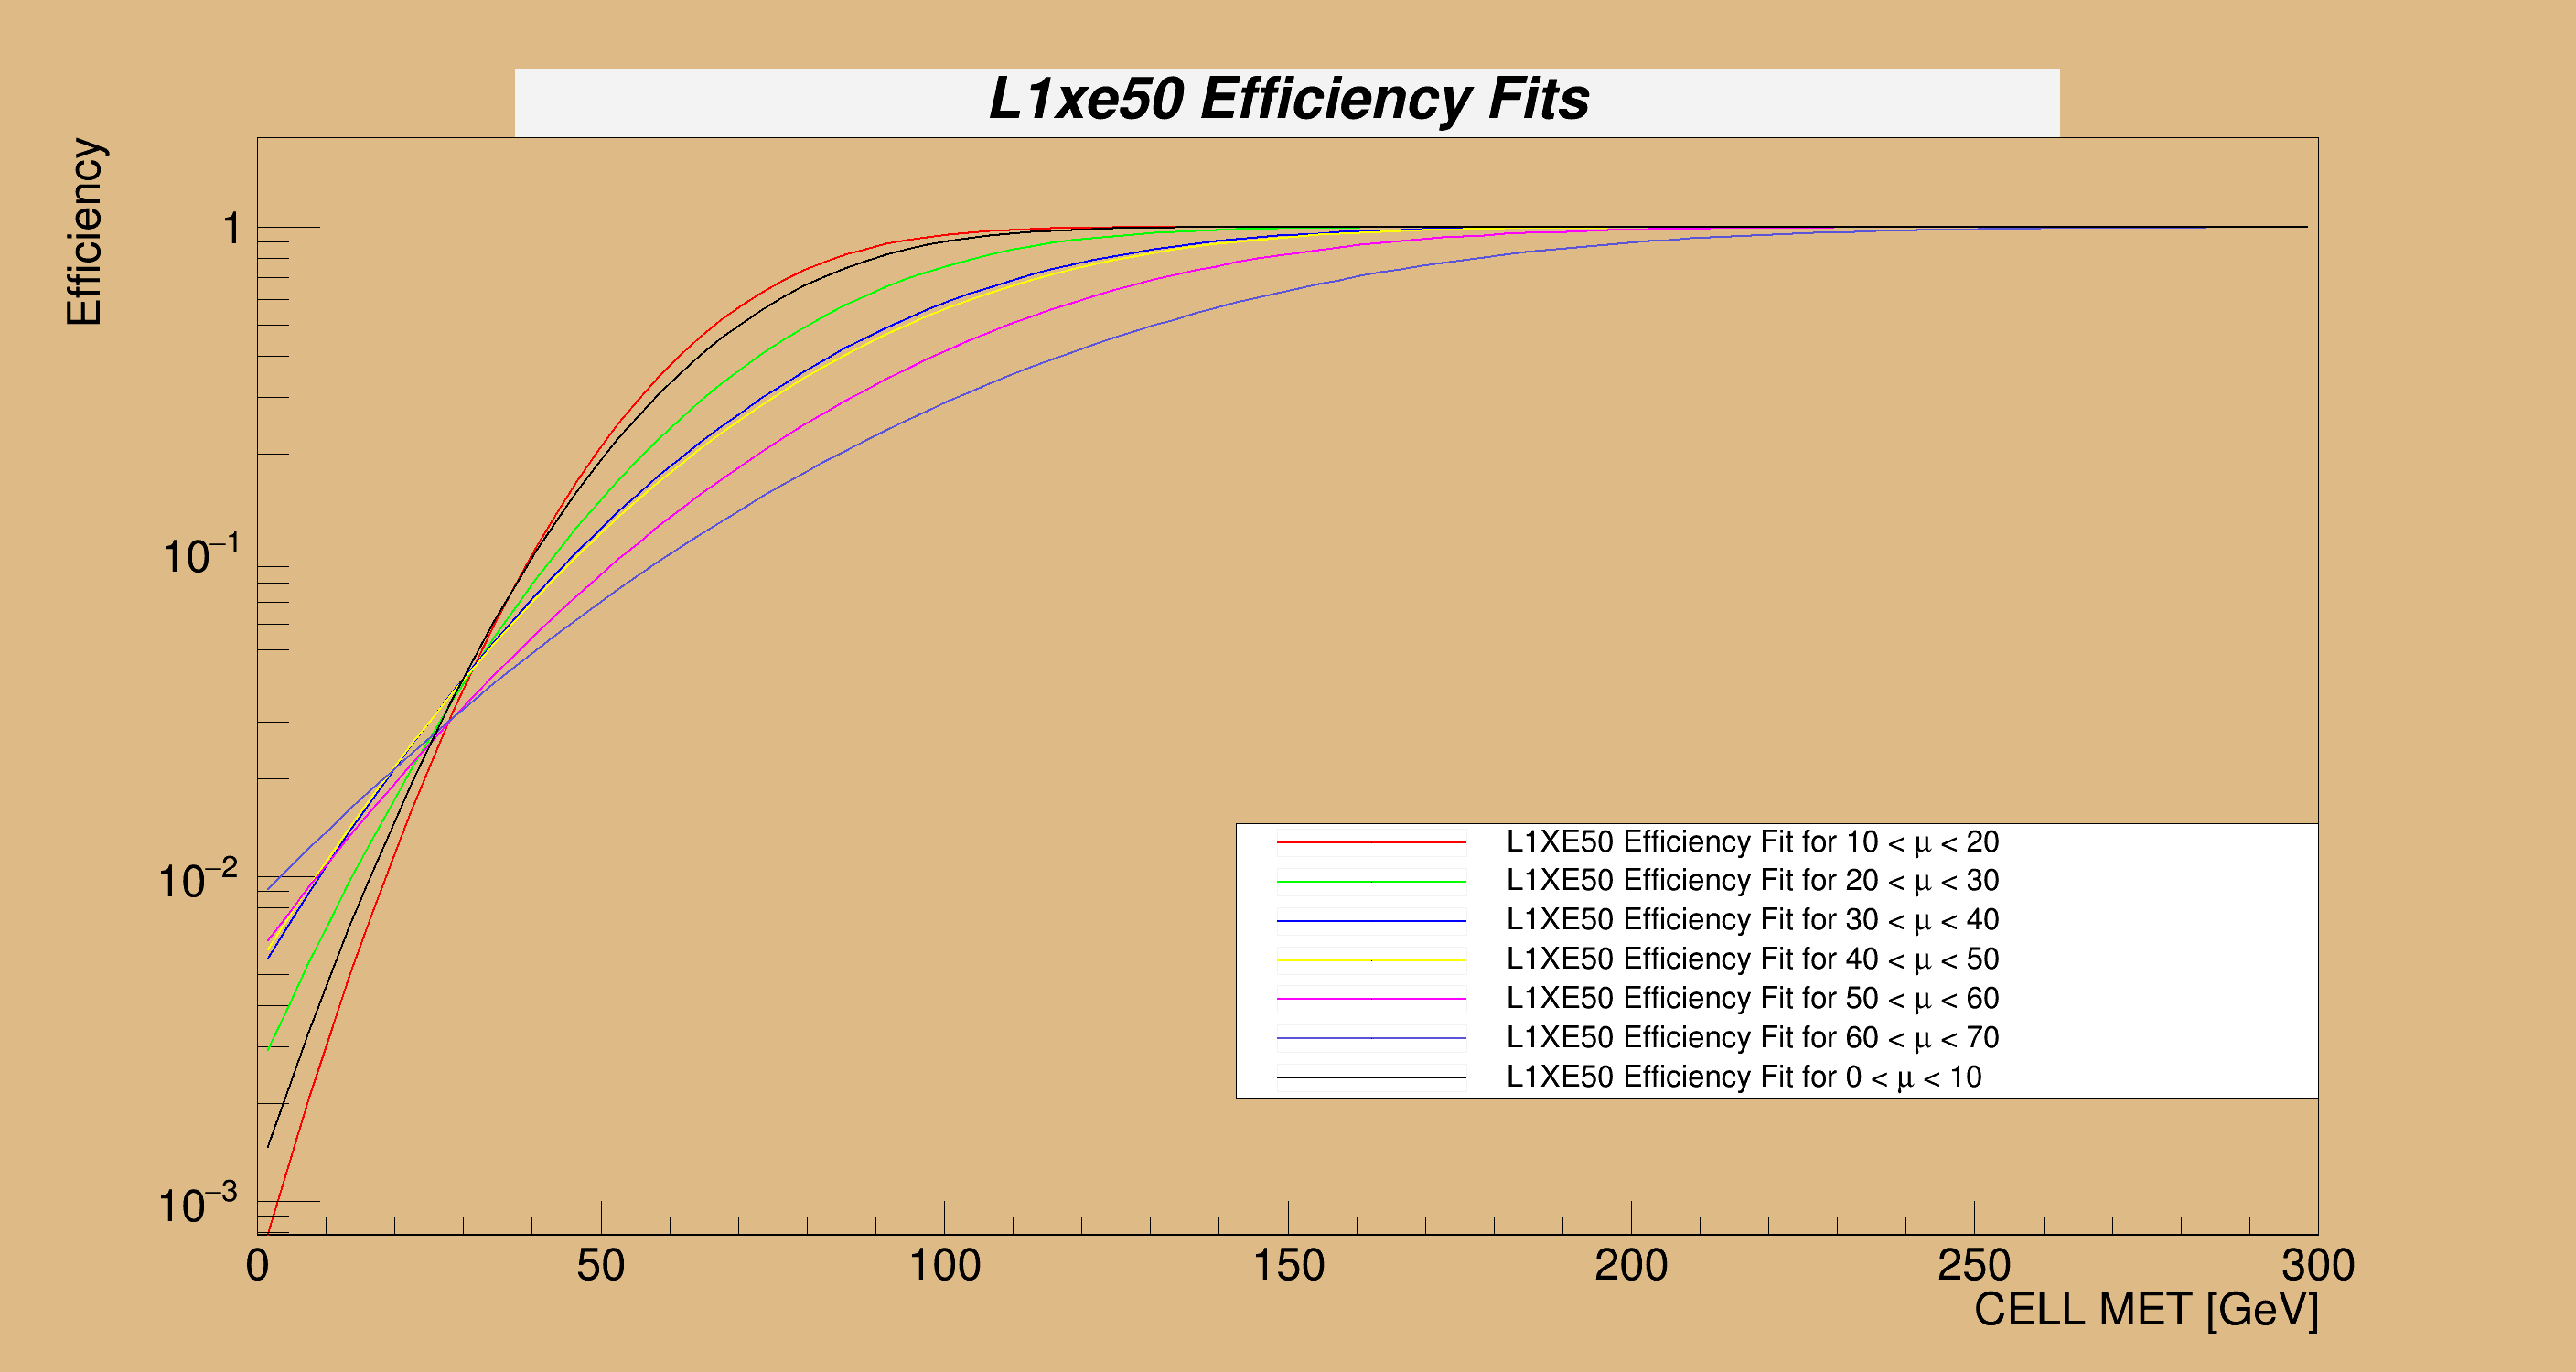
\includegraphics[scale=0.15]{L1XE50Efficiency_Fits}
		\caption{Efficiency Fits of L1$>50$ on the \texttt{HLT\_noalg\_L1XE30} data}
\end{figure}
\clearpage
\section{Error Propagation}
In order to obtain accurate error bars on the bins of our reconstructed distribution, it was necessary to appropriately propagate errors due to the determination of the efficiency and the statistical error. 
Because the value of the prescale varies within a given bin, it was necessary to keep track of the error accumulated on a particular bin manually. 
In order to do this, the formula for propagation of fractional uncertainties was used. 
We have the fact that the expression for what the contribution from a single event to the current bin should look like is given by:
\begin{align}
		n_{ZB}^{30}=\frac{P_{30}}{\varepsilon_{ZB}^{30}}\cdot n
\end{align}
\begin{align}
		\left(\frac{\delta n_{ZB}^{30}}{n_{ZB}^{30}}\right)^2&=\left( \frac{\delta P_{30}}{P_{30}} \right)^2+\left( \frac{\delta \varepsilon_{ZB}^{30}}{\varepsilon_{ZB}^{30}} \right)^2+\left( \frac{\delta n}{n} \right)^2\\
		&=\left( \frac{\delta \varepsilon_{ZB}^{30}}{\varepsilon_{ZB}^{30}} \right)^2+1
\end{align}
Because we know the prescale exactly, we have that $\delta P_{30}=0$ and $\delta P_{50}=0$, so those terms drop out.
Because this is a single event, we have that $n=1$ and by the standard deviation of a poisson process $\delta n=\sqrt{n}$, which means that $\delta n=1$. So the term due to statistical uncertainty contributes unity on the right hand side.
In addition to computing the uncertainty on the contribution of a single event with given prescale and efficiency during the correction of the \texttt{HLT\_noalg\_L1XE30} data to the unbiased distribution, we need to also know the uncertainty on the correction of a given event from the \texttt{HLT\_noalg\_L1XE50} data to the unbiased distribution.
In order to compute the unbiased distribution from the \texttt{HLT\_noalg\_L1XE50} events, it was necessary to multiply a given event by its recorded prescale ($P_{50}$), as well as divide by both the efficiency of the \texttt{HLT\_noalg\_L1XE50} data relative tot he \texttt{HLT\_noalg\_L1XE30} data, and the efficiency of the \texttt{HLT\_noalg\_L1XE30} data to the \texttt{HLT\_noalg\_L1ZB} data.
\begin{align}
		n_{ZB}^{50}=\frac{P_{50}}{\varepsilon_{ZB}^{30}\varepsilon_{ZB}^{50}}\cdot n
\end{align}
\begin{align}
		\left(\frac{\delta n_{ZB}^{50}}{n_{ZB}^{50}}\right)^2&=\left( \frac{\delta P_{50}}{P_{50}} \right)^2+\left( \frac{\delta \varepsilon_{ZB}^{30}}{\varepsilon_{ZB}^{30}} \right)^2+\left( \frac{\delta \varepsilon_{ZB}^{50}}{\varepsilon_{ZB}^{50}} \right)^2+1\\
&=\left( \frac{\delta \varepsilon_{ZB}^{30}}{\varepsilon_{ZB}^{30}} \right)^2+\left( \frac{\delta \varepsilon_{ZB}^{50}}{\varepsilon_{ZB}^{50}} \right)^2+1
\end{align}
I track of these uncertainties by incrementing the elements of an array that corresponded to the square error of that bin of the histogram, and taking the square root at the end to get the numeric value for the uncertainty on that bin for both of the corrected distributions.\\
In order to compute the factors $\varepsilon_{ZB}^{30}$ and $\varepsilon_{ZB}^{50}$, it was necessary to propagate errors in quadrature. The expression for this computation is given by:
\begin{align}
		(\delta \varepsilon)^2=\sum_{i=1}^k\left( \delta \theta_i \frac{\partial f}{\partial \theta_i} \right)^2
\end{align}
where $k$ is the number of parameters in the fitting function we used, $f$ is the fitting function we used, and $\theta_i$ is the $i$th parameter.
After some manipulation with partial derivatives and exponential integrals, one can derive that the expression for $\delta \varepsilon_{ZB}^{30}$ is given by:
\begin{align}
		\delta \varepsilon_{ZB}^{30}=\sqrt{\frac{1}{2\pi\sigma^2}}\textrm{exp}\left(-\left( \frac{ax+b-30}{\sqrt{2}\sigma} \right)^2\right)\left[ \delta a^2x^2+\delta b^2 +\delta \sigma^2 \left( \frac{ax+b-30}{\sigma} \right)^2 \right]^{1/2}
\end{align}

\section{Relative Normalization}
Because the error bars are larger at lower values of MET, it is necessary to also perform an overall relative normalization between the \texttt{HLT\_noalg\_L1XExx} data and the \texttt{HLT\_noalg\_L1ZB} data in addition to the normalization to unity.
This was done in order to compare the shapes of the curves more easily.
The relative normalization factor was computed by taking a weighted average of ratios sampled at various points in the tail of the distribution where the slopes of the distributions were approximately parallel.
The expression for the relative normalization factor is given by:
\begin{align}
		\hat{f}_{MLE}=\frac{\sum_{i=1}^k \frac{1}{\sigma_i^2}f_i}{\sum_{i=1}^k \frac{1}{\sigma_i^2}}
\end{align}
where $k$ is the number of samples taken from the tail of the distribution in the region where the slopes were approximately parallel.
Using the expression for the propagation of fractional uncertainty, one can calculate the error in this expression for the relative normalization factor:
\begin{align}
		\sigma_i(f_i)=f_i\sqrt{\left( \frac{\sigma_{ZB}^{50}}{N_{ZB}^{50}} \right)^2+\left(\frac{\sigma_{ZB}}{N_{ZB}}\right)^2}
\end{align}
Note that in this case, we are not propagating the error on a single event, but on a given ratio of bin values. 
The variables are: $\sigma_{ZB}^{50}$ is the error on the given bin from the \texttt{HLT\_noalg\_L1XE50} distribution after being corrected to the unbiased distribution, the $N_{ZB}^{50}$ is the value of that bin, and the $\sigma_{ZB}$ is the error on the corresponding bin from the \texttt{HLT\_noalg\_L1ZB} distribution and $N_{ZB}$ is the number of events in that bin.
